\section{Complex network theory} \label{sec:CompNetworkT}
In this section, we provide the brief introduction of the characterization of structural properties of a network, focusing on definitions, notations, and basic quantities that are often used to describe the topologies of networks reconstructed from time series. More comprehensive descriptions of complex networks can be found in a number of review articles \cite{Albert2002,Newman2003,Boccaletti2006,Costa2007} and books \cite{Cohenbook2010,Newmanbook2010}, which the reader may find useful to consult.  
	
	
	\subsection{Basic concepts} \label{sec:basicCompNets}
	A complex network is often represented as a graph $G = (V, E)$ which consists of two sets $V$ and $E$, where $V$ is the set of vertices (nodes or points) of $G$, and $E$ is the set of edges (links or lines) representing pairs of connected elements of $V$ \cite{Costa2007}. Each vertex is identified by an integer index $p=1,\dots,N$, and each edge is identified by a pair $(p,q)$ connecting two vertices $p$ and $q$. A graph $G$ is called undirected if an edge from vertex $p$ to $q$ as denoted by $(p,q)$ is equivalent to the edge of $(q,p)$ from vertex $q$ to $p$, i.e., $(p,q)\in E \Leftrightarrow (q,p)\in E$. On the other hand, in a directed graph, typically $(p,q)\in E \nLeftrightarrow (q,p)\in E$. A graph may contain loops, i.e., edges from a vertex to itself, or multiple edges, i.e., pairs of vertices connected by more than one edge. 
    
    More generally, edges $(p,q)$ may be attributed additional weights $W_{pq}$. For convenience, one commonly defines $W_{pq}=0$ of $(p,q)\notin E$, In this case, a weighted directed graph can be completely described by its weight matrix $\mathbf{W}$ so that each entry $W_{pq}$ expresses the weight of the connection from vertex $p$ to vertex $q$. In this section, we only consider undirected and unweighted graphs for the sake of simplicity, since there is no need for discussing $W_{pq}$ in the context of most of the complex network approaches for time series analysis discussed in this review. A notable exception from this are transition networks, for which Weighted graphs will receive a special attention in Section \ref{sec:TransitionNt}. 
	
	An unweighted graph can be naturally constructed by applying a proper threshold $T$ to the elements of the weight matrix $\mathbf{W}$ of its weighted counterpart \cite{Costa2007}, resulting in the binary matrix $\mathbf{A}$. Specifically, we have $A_{pq} = 1$ if $W_{pq} > T$, otherwise, $A_{pq} = 0$. The resulting matrix $\mathbf{A}$ is called the \emph{adjacency matrix} of the resulting unweighted graph, and each nonzero element $A_{pq}$ of $\mathbf{A}$ indicates the presence of $(p,q)$ as a member of its edge set $E$. Further introduction of symmetry to $\mathbf{A}$, i.e., identifying $A_{pq} = A_{qp}$, is characteristic of an undirected graph. Such an undirected, unweighted graph is also called a simple graph.  
	
	Depending on the particular mappings for transforming a given time series into a complex network, the resulting adjacency matrix $\mathbf{A}$ often depends on some algorithmic parameters, for instance, the threshold value $\varepsilon$ of the recurrence network approach (Section~\ref{sec:RecurrenceNt}). More importantly, we often have some particular interpretations for network measures, for instance, in terms of the geometry of a dynamical system. In the following, we first introduce some general measures for characterizing some important aspects of network structures based on $\mathbf{A}$. More specific discussions of network measures in terms of the particular network transforming methods will be presented in later sections. 

	In addition to the concepts of vertices and edges, another important concept in complex network theory is the notion of paths. A \emph{path} between two specified vertices $p$ and $q$ is an ordered sequence of edges starting at $p$ and ending at $q$, with its \emph{path length} $l_{pq}$ given by the number of edges in this sequence. There are also various measures characterizing the structural properties of networks based on paths, which will be briefly reviewed here as well.  

	\subsection{Network characteristics} \label{sec:basictheoryCN}
		\subsubsection{Vertex characteristics}
		There are various measures to characterize the structures of a complex network, quantifying the importance of either a vertex or an edge in terms of a particular network property. The conceptually simplest measure characterizing the connectivity properties of a single vertex in a complex network is the \textit{degree} (or \textit{degree centrality})
\begin{equation} 
k_p=\sum_{q=1}^N A_{pq} ,
\label{eq:degree}
\end{equation}
\noindent
which simply counts the number of edges associated with a given vertex $p$. It is also convenient to introduce a normalized degree 
\begin{equation} \label{eq:localrho}
\rho_p = \frac{1}{N-1} k_p
\end{equation}
as the local connectivity density of $p$. Furthermore, a topological characterization of the graph $G$ as a whole can be obtained in terms of the degree distribution $p(k)$, defined as the probability that a vertex chosen uniformly at random has degree $k$ or, equivalently, as the fraction of vertices in the graph having degree $k$. Note that the variable $k$ assumes non-negative integer values. The degree distribution $p(k)$ is often used to classify complex networks, for instance, a scale-free network is characterized by $p(k) \sim k^{-\gamma}$, which will further discussed in Sec. \ref{sec:styleFacts}. Furthermore, one simple definition of a network entropy  is based on the degree distribution as $S = - \sum_{k} p(k) \log p(k)$, which can be computed straightforwardly \cite{Rashevsky1955,MacArthur1955}. A more recent survey of information theoretic measures based on different network partitions of complex topology has been presented in \cite{Dehmer2011}. 

		In order to characterize the density of connections among the neighbors of a given vertex $p$, we can utilize the \textit{local clustering coefficient}
\begin{equation}
  {\mathcal{C}}_p =\frac{1}{  {k}_p (  {k}_p -1)} \sum_{q,r=1}^N A_{pq}  A_{qr}  A_{rp} ,
\label{eq:locclustering}
\end{equation}
\noindent
which measures the fraction of pairs of vertices in the neighborhood of $p$ that are mutually connected. 

		While degree and local clustering coefficient characterize network structures on the local and meso-scale, there are further vertex characteristics that make explicit use of the concept of shortest paths and, thus, provide measures relying on the connectivity of the entire network. Two specific properties of this kind are the \textit{closeness} or \textit{closeness centrality}
\begin{equation}
  {c}_p =\left(\frac{1}{N-1}\sum_{q=1}^N   {l}_{pq}  \right)^{-1},
\label{eq:closeness}
\end{equation}
\noindent
which gives the inverse arithmetic mean of the shortest path lengths $l_{pq}$ between vertex $p$ and all other vertices $q\in V$, and the \textit{local efficiency}
\begin{equation}
  {e}_p =\frac{1}{N-1}\sum_{q=1}^N   {l}_{pq} ^{-1},
\label{eq:locefficiency}
\end{equation}
\noindent
which gives the inverse harmonic mean of these shortest path lengths. Notably, the latter quantity has the advantage of being well-behaved in the case of disconnected network components, where there are no paths between certain pairs of vertices (i.e., $  {l}_{pq}=\infty$). In order to circumvent divergences of the closeness due to the existence of disconnected components, it is convenient to always set ${l}_{pq}$ to the highest possible value of $N-1$ for pairs of vertices that cannot be mutually reached. Both $  {c}_p $ and $  {e}_p $ characterize the geometric centrality of vertex $p$ in the network, i.e., closeness and local efficiency exhibit the highest values for such vertices which are situated in the center of the networks. 

		Another frequently studied path-based vertex characteristic is the \textit{betweenness} or \textit{betweenness centrality}, which measures the fraction of shortest paths in a network traversing a given vertex $p$. Let $  {\sigma}_{qr}$ denote the total number of shortest paths between two vertices $q$ and $r$ and $  {\sigma}_{qr}(p)$ the multiplicity of these paths that include a given vertex $p$, betweenness centrality is defined as
\begin{equation}
  {b}_p =\sum_{q,r=1; q,r\neq p}^N \frac{  {\sigma}_{qr}(p)}{  {\sigma}_{qr}}.
\label{eq:betweenness}
\end{equation}
\noindent
It is commonly used for characterizing the importance of vertices for information propagation in networks. 

		\subsubsection{Edge characteristics}
		In contrast to vertices, whose properties can be characterized by a multitude of graph characteristics, there are fewer measures that explicitly relate to the properties of edges or, more general, pairs of vertices. One such measure is the \textit{matching index}, which quantifies the overlap of the network neighborhoods of two vertices $p$ and $q$:
\begin{equation}
  {m}_{pq} =\frac{\sum_{r=1}^N A_{pr}  A_{qr} }{  {k}_p +  {k}_q -\sum_{r=1}^N A_{pr}  A_{qr} }.
\label{eq:matching}
\end{equation}
\noindent

		While the concept of matching index does not require the presence of an edge between two vertices $p$ and $q$, there are other characteristics that are explicitly edge-based. To this end, we only mention that the concept of betweenness centrality $b_p$ can also be transferred to edges, leading to the \textit{edge betweenness} measuring the fraction of shortest paths on the graph traversing through a specific edge $(p,q)$:
\begin{equation}
  {b}_{pq} =\sum_{r,s=1; r,s\neq p,q}^N \frac{  {\sigma}_{rs}(p,q)}{  {\sigma}_{rs}},
\label{eq:edgebetweenness}
\end{equation}
\noindent
where $  {\sigma}_{rs}(p,q)$ gives the total number of shortest paths between two vertices $r$ and $s$ that include the edge $(p,q)$. If there is no edge between two vertices $p$ and $q$, we set $  {b}_{pq}=0$ for convenience. 
        
        		Finally, we mention the concept of network motifs \cite{Milo2002} as another edge-based way to obtain proper information on the meso-scale connectivity properties of a graph, which generalize the idea of the local clustering coefficient and are particularly useful for the study of directed networks. In this context, motifs are small connected subgraphs consisting of a small fixed number of vertices (typically, 3 or 4 due to their fastly increasing combinatorial variety and computational demanding), which represent specific local connection patterns that allow classifying real-world networks into superfamilies according to the relative frequencies of different motifs \cite{Milo2002}. In terms of time series networks, we focus on the frequency distribution of motifs which may serve as a sensitive indicator of specific type of network structures that are reconstructed by different methods, for instance, in Section \ref{sec:adaptiveRN}. 
		        
        		\subsubsection{Global network characteristics}
		Some, but not all useful global network characteristics can be derived by averaging certain local-scale (vertex) properties. Prominently, the \textit{edge density}
\begin{equation}
  {\rho} =\frac{1}{N}\sum_{p=1}^N   {\rho}_p =\frac{1}{N(N-1)} \sum_{p,q=1}^N A_{pq} 
\label{eq:edgedensity}
\end{equation}
is defined as the arithmetic mean of the degree densities of all vertices $\rho_p$ and characterizes the fraction of possible edges that are present in the network. 

		In a similar way, we consider the arithmetic mean of the local clustering coefficients $  {\mathcal{C}}_p $ of all vertices, resulting in the (Watts-Strogatz) \textit{global clustering coefficient}~\cite{Watts1998}
\begin{equation}
  {\mathcal{C}} =\frac{1}{N}\sum_{p=1}^N   {\mathcal{C}}_p 
= \frac{1}{N}\sum_{p=1}^N \frac{\sum_{q,r=1}^N A_{pq}  A_{qr}  A_{rp} }{  {k}_p (  {k}_p -1)}, 
\label{eq:globclustering}
\end{equation}
which measures the mean fraction of triangles that include the different vertices of the network. 

		Notably, in the case of a very heterogeneous degree distribution, the global clustering coefficient will be dominated by contributions from the most abundant type of vertices, the hubs. For example, for a scale-free network with $p(k)\sim k^{-\gamma}$, vertices with small degree will contribute predominantly, which can lead to an underestimation of the actual fraction of triangles in the network, since $  {\mathcal{C}}_p =0$ if $  {k}_p <2$ by definition. In order to correct for such effects, Barrat and Weigt~\cite{Barrat2000} proposed an alternative definition of the clustering coefficient, which is nowadays frequently referred to as \textit{network transitivity}~\cite{Boccaletti2006} and is defined as
\begin{equation}
  {\mathcal{T}} = \frac{\sum_{p,q,r=1}^N A_{pq}  A_{qr}  A_{rp} }{\sum_{p,q,r=1}^N A_{pq}  A_{rp} }.
\label{eq:transitivity}
\end{equation}
\noindent

	Finally, turning to shortest path-based characteristics, we define the \textit{average path length}
\begin{equation}
  {\mathcal{L}} =\frac{1}{N(N-1)} \sum_{p,q=1}^N   {l}_{pq}  = \frac{1}{N} \sum_{p=1}^N   {c}_p ^{-1}
\label{eq:apl}
\end{equation}
\noindent
as the arithmetic mean of the shortest path lengths between all pairs of vertices, and the \textit{global efficiency}
\begin{equation} 
  {\mathcal{E}} =\left(\frac{1}{N(N-1)} \sum_{p,q=1}^N   {l}_{pq} ^{-1} \right)^{-1} = \left( \frac{1}{N} \sum_{p=1}^N   {e}_p  \right)^{-1}
\label{eq:globefficiency}
\end{equation}
\noindent
as the associated harmonic mean. Notably, the average path length can be rewritten as the arithmetic mean of the inverse closeness, and the global efficiency as the inverse arithmetic mean of the local efficiency. Furthermore, based on shortest path length, one often defines the diameter of a network as the longest (maximum) of all the calculated shortest paths in a network, $\mathcal{D} = \max_{p,q} l_{pq}$. In other words, once the shortest path length from every vertex to all other vertices is calculated, the diameter $\mathcal{D}$ is the maximum of all the calculated path lengths. Certainly, the diameter is representative of the size of a network.       

	\subsection{Stylized facts of complex networks} \label{sec:styleFacts}
	Erd\"os and R\'enyi \cite{Erdos1959} introduced a model to generate random graphs consisting of $N$ vertices and $M$ edges. Starting with $N$ disconnected vertices, the network is constructed by the addition of $L$ edges at random, avoiding multiple and self connections. Another similar model defines $N$ vertices and a probability $p$ of connecting each pair of vertices. The latter model is widely known as the Erd\"os-R\'enyi (ER) model. For the ER model, in the large network size limit $(N \to \infty)$, the average number of connections of each vertex $\left < k \right>$ is given by $\left< k \right > = c (N - 1)$, where $c$ is fixed and often chosen as a function of $N$ to keep $\left < k \right >$ fixed. For this model, the degree distribution $p(k)$ is a Poisson distribution. 
	
	In regular hypercubic lattices in $d$ dimensions, the mean number of vertices one has to pass in order to reach an arbitrarily chosen vertex, grows with the lattice size as $N^{1/d}$. Conversely, in most real-world networks, despite of their often large size $N$, there is a relatively short path between any two vertices. This property, which is shared by many real-world networks, is the so-called small-world (SW) effect, that has been first described as the outcome of studies on social interrelationships, predominantly Milgram's famous chain-letter experiment in the 1960s \cite{Milgram1967}. In the spirit of the latter studies, the term ``SW effect'' originally denoted the fact that average shortest path lengths $\mathcal{L}$ (Eq.~\ref{eq:apl}) in social networks, but also other real-world networks, are much shorter than we would expect from random connectivity configurations. Given the importance of redundancy in such networks, Watts and Strogatz \cite{Watts1998} suggested including the presence of a high clustering coefficient $\mathcal{C}$ (i.e., higher than in random graphs) as a second criterion for identifying the small-world effect in real-world networks. According to their definition, small-world networks are characterized by having both a small value of $\mathcal{L}$, like random graphs, and a high clustering coefficient $\mathcal{C}$, like regular lattices. The generative model introduced by them (WS model) is based on a probabilistic rewiring of edges in a regular ring lattice (i.e., each existing edge is rewired uniformly at random with the same probability $c$) and is thus situated between an ordered finite lattice ($c=0$) and a random graph ($c=1$), presenting the small world property with short path length and high clustering coefficient at intermediate values of $c$. 

	Barab\'asi and Albert \cite{Barabasi199} showed that the degree distribution $p(k)$ of many real-world systems is characterized by a heavy-tailed distribution. Instead of the vertices of these networks having a random pattern of connections with a characteristic degree, as in the ER and WS models, some vertices are highly connected while others have few connections, with the absence of a characteristic degree. More specifically, the degree distribution has been found to follow a power-law for large $k$, $p(k) \sim k^{-\gamma}$. These networks are called scale-free (SF) networks, which are captured by a pronounced linear regime in the double logarithmic plot of $p(k)$. In order to model the emergence of such network structures, the BA model has been proposed which contains the two important ingredients of network growth and preferential attachment. A proper statistical identification of SF properties in real-world networks is a non-trivial task because of effects originating from finite size, intrinsic noise and finite sample size \cite{Clauset2009}. 
	
	In addition, a large number of real-world networks are correlated in the sense that the probability that a node of degree $k$ is connected to another node of degree, say $k'$, depends on $k$. This problem can be quantified by the average nearest neighbor degree of a vertex $p$, or, alternatively, the assortativity coefficient $\mathcal{R}$, i.e., the correlation coefficient between the degrees of all pairs of mutually connected vertices \cite{Newman2002}. In assortative networks, the vertices tend to connect to their connectivity peers ($\mathcal{R} > 0$), while in disassortative networks vertices with low degrees are more likely connected with highly connected ones ($\mathcal{R} < 0$). 
	
	In the following sections, the presence or absence of these stylized facts of complex networks will be discussed in the respective frameworks when introducing different network construction algorithms based upon possibly nonlinear time series. 
	
		\subsection{Multiplex and multilayer networks} \label{sec:multiplex}
			%\subsubsection{General introduction}
			Many complex systems include multiple subsystems and layers of connectivity and they evolve, adapt and transform through internal and external dynamical interactions affecting the subsystems and components at both local and global scale. For example, the problem of information or rumor spreading on top of a social network like Facebook must take into account the intricate interactions on different levels \cite{Boccaletti2014}. In general, many interactions in social networks can be understood as a combination of interactions at different, independent levels, each representing different social scenarios such as family, friends, coworkers, etc. The actual relationships amongst the members of a social network must consider interactions mostly inside the levels and their influences on the other layers. An individual's behavior can be different in each level but it is conditioned by other levels. Multiplex and multilayer networks explicitly incorporate multiple levels of social interactions and have been successfully applied to the study of disease spreading and diffusion dynamics \cite{Gomez2013,Granell2013} or the evolution of cooperation in the presence of social dilemmas  \cite{Matamalas2015}. 
			
			Understanding and possibly predicting multi-scale and multi-component dynamics is a difficult challenge to complex systems theory \cite{Boccaletti2014}. In this context, the issues posed by the multi-scale modeling of both natural and artificial complex systems call for a generalization of the ``traditional" network theory, foremost including the development of a solid theoretical foundation and associated tools for studying multilayer and multi-component systems in a comprehensive fashion. 
		
			Here, we follow the formal definition of a {\textit{multilayer network}} \cite{Boccaletti2014} as a pair $\mathcal{M} = (\mathcal{G}, \mathcal{C})$ where $\mathcal{G} = \{G_{\alpha}; \alpha=1, \dots, M\}$ is a family of graphs $G_{\alpha} = (V_{\alpha}, E_{\alpha})$ and 
		\begin{equation}
		\mathcal{C} = \{ E_{\alpha\beta} \subseteq V_{\alpha} \times V_{\beta}; \alpha, \beta \in [1, 2, \dots, M], \alpha \neq \beta \}
		\end{equation}
		is the set of interconnections between nodes of different layers $G_{\alpha}$ and $G_{\beta}$ with $\alpha \neq \beta$. The elements of each $E_{\alpha}$ are called intra-layer connections of $\mathcal{M}$ as opposed to those of each $E_{\alpha\beta}$ with $\alpha\neq\beta$ that are called inter-layer connections. By using the multilayer network representation, we simultaneously consider edges that are located inside different layers and such that connect different layers. A {\textit{multiplex network}} is a special type of multilayer network in which each layer shares the same set of vertices, i.e., $V_{1} = \dots = V_M$, and the only possible type of interlayer connections are those in which a given node is connected to its counterparts in the other layers.  In other words, a multiplex network consists of a fixed set of vertices connected by different types of edges \cite{Boccaletti2014}. 
		
			The readers are referred to \cite{Boccaletti2014,Buldyrev2010} for a more thorough review on multilayer networks. Furthermore, it is important to remark that the concept of multilayer networks has been extended to other relevant notations, for instance, network of networks, interacting or interconnected networks, multidimensional networks, interdependent networks, multilevel networks, hypernetworks, etc., some of which are used as synonyms of each other. 	
	
		\subsection{Coupled networks}\label{sec:irn_measures}
	    		
                \subsubsection{Preliminaries}
			When describing multilayer and multiplex networks in Section \ref{sec:multiplex}, we have introduced a corresponding rather general framework. In the particular case of networks constructed from two or more possibly interdependent time series, different perspectives can be taken with respect to the coupled system. Under some conditions, it can be preferable to utilize the recently introduced framework of coupled or interdependent network analysis for a corresponding topological characterization \cite{Donges2011b,Wiedermann2013}. The study of coupled networks focuses on interrelationships between the different subnetworks, i.e., on a dependency scenario in which vertices in one network require connections to vertices in another subnetwork (e.g., in case of telecommunication networks and power grids) \cite{Buldyrev2010}. 
			
			Let us again consider an arbitrary undirected and unweighted simple graph $G=(V,E)$ with the adjacency matrix $\textbf{A}=\{A_{pq}\}_{p,q=1}^N$. Furthermore, let us assume that there is a given partition of $G$ with the following properties:
\begin{enumerate}
\item The vertex set $V$ is decomposed into $M$ disjoint subsets $V_\alpha \subseteq V$ such that $\bigcup_{\alpha=1}^M V_\alpha = V$ and $V_\alpha \cap V_\beta = \emptyset$ for all $\alpha \neq \beta$. The cardinality of $V_\alpha$ will be denoted as $N_\alpha$. 

\item The edge set $E$ consists of mutually disjoint sets $E_{\alpha\beta} \subseteq E$ with $\bigcup_{\alpha,\beta=1}^K E_{\alpha\beta} = E$ and $E_{\alpha\beta} \cap E_{\gamma\delta}=\empty$ for all $(\alpha,\beta) \neq (\gamma,\delta)$.

\item Let $E_{\alpha\beta}\subseteq V_\alpha \times V_\beta$. Specifically, for all $\alpha=1,\dots,M$, $G_\alpha=(V_\alpha,E_{\alpha\alpha})$ is the induced subgraph of the vertex set $V_\alpha$ with respect to the full graph $G$.
\end{enumerate}
Under these conditions, $E_{\alpha\alpha}$ comprises the (internal) edges within $G_\alpha$, whereas $E_{\alpha\beta}$ contains all (cross-) edges connecting $G_\alpha$ and $G_\beta$. 

			We are now in a position to study the interconnectivity structure between two subnetworks $G_\alpha, G_\beta$ on several topological scales drawing on the lineup of local and global graph-theoretical measures generalizing those used for single network characterization (see Section~\ref{sec:IntSRN}). In this context, local measures ${f}_p^{\alpha\beta}$ characterize a property of vertex $p \in V_\alpha$ with respect to subnetwork $G_\beta$, while global measures ${F}^{\alpha\beta}$ assign a single real number to a pair of subnetworks $G_\alpha, G_\beta$ to quantify a certain aspect of their mutual interconnectivity structure. Most interconnectivity characteristics discussed below have been originally introduced in \cite{Donges2011b}.

			\subsubsection{Vertex characteristics}
			The \textit{cross-degree} (or \textit{cross-degree centrality})
\begin{equation}
{k}_p^{\alpha\beta} = \sum_{q \in V_\beta} A_{pq}
\label{eq:degree_cross}
\end{equation}
counts the number of neighbors of vertex $p \in V_\alpha$ within the subnetwork $G_\beta$, i.e., direct connections between $G_\alpha$ and $G_\beta$ (Fig.~\ref{fig:interacting_measures}A). Thus, this measure provides information on the relevance of $p$ for the network ``coupling'' between $G_\alpha$ and $G_\beta$. For the purpose of the present work, it is useful studying a normalized version of this measure, the \textit{cross-degree density}
\begin{equation}
{\rho}_p^{\alpha\beta} = \frac{1}{N_\beta} \sum_{q \in V_\beta} A_{pq} = \frac{1}{N_\beta} {k}_p^{\alpha\beta}.
\label{eq:locrho_cross}
\end{equation}

\begin{figure}
	\centering
	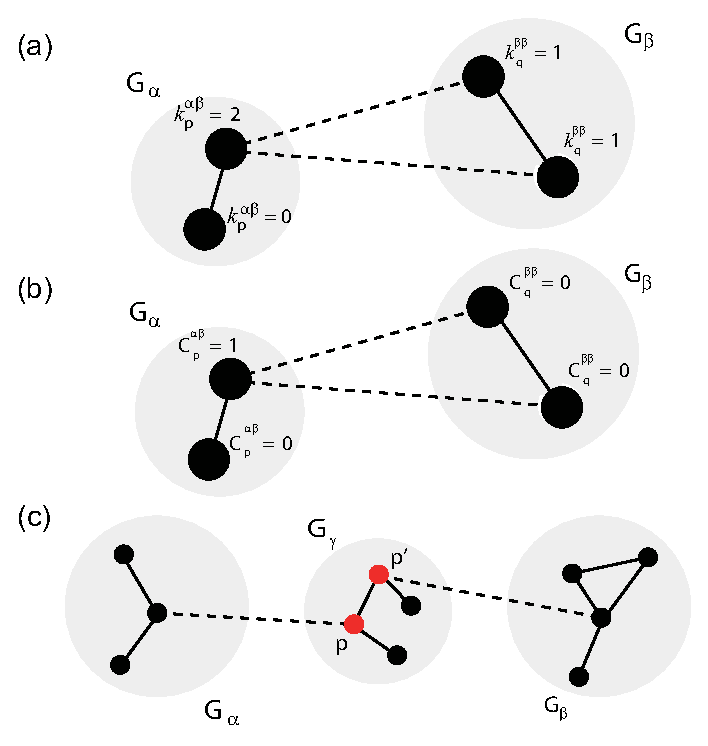
\includegraphics[scale=0.8]{Chapter02_CompNetworkT/cross_measures_schematic.eps} 
\caption{Schematic illustration of some characteristics of interdependent networks: (a) The cross-degree $k_p^{\alpha\beta}$ (Eq.~\eqref{eq:degree_cross}). In the example $\rho^{\alpha\beta}=0.5$. (b) The local cross-clustering coefficient $\mathcal{C}_p^{\alpha\beta}$ (Eq.~\eqref{eq:locclustering_cross}). In the example, the associated values are $\mathcal{C}^{\alpha\beta}=0.5$ and $\mathcal{C}^{\beta\alpha}=0$, whereas $\mathcal{T}^{\alpha\beta}=1$ and $\mathcal{T}^{\beta\alpha}=0$. (c) The cross-betweenness centrality $b_p^{\alpha\beta}$ (Eq. \eqref{eq:betweenness_cross}). In the example, $p,q\in V_\gamma$ (red) have a large cross-betweenness, whereas the remaining vertices $p\in V_\gamma\setminus\{p,q\}$ from subnetwork $G_\gamma$ do not participate in shortest paths between $G_\alpha$ and $G_\beta$ and therefore have vanishing values $b_r^{\alpha\beta}=0$. Modified from \cite{Donges2012PhD,Donges2011b}. } \label{fig:interacting_measures}
\end{figure}

		As for the single network case, important information is governed by the presence of triangles in the network. Given two subnetworks, the \textit{local cross-clustering coefficient}
\begin{equation}
{\mathcal{C}}_p^{\alpha\beta} = \frac{1}{{k}_p^{\alpha\beta}({k}_p^{\alpha\beta} - 1)} \sum_{q,r \in V_\beta} A_{pq} A_{qr} A_{rp},
\label{eq:locclustering_cross}
\end{equation}
\noindent
measures the relative frequency of two randomly drawn neighbors $q,r\in V_\beta$ of $p\in V_\alpha$ are mutually connected (Fig.~\ref{fig:interacting_measures}B). For ${k}_p^{\alpha\beta}<2$, we define ${\mathcal{C}}_p^{\alpha\beta}=0$. In general, ${\mathcal{C}}_p^{\alpha\beta}$ characterizes the tendency of vertices in $G_\alpha$ to connect to clusters of vertices in $G_\beta$. 

		The \textit{cross-closeness centrality}
\begin{equation}
{c}_p^{\alpha\beta} = \left(\frac{\sum_{q \in V_\beta} l_{pq}}{N_\beta}\right)^{-1}
\label{eq:closeness_cross}
\end{equation}
\noindent
(where $l_{pq}$ is the shortest-path length between $p$ and $q$) characterizes the topological closeness of $p\in G_\alpha$ to $G_\beta$, i.e., the inverse arithmetic mean of the shortest path lengths between $p$ and all vertices $q\in V_\beta$. If there exist no such paths, $l_{pq}$ is commonly set to the maximum possible value $N-1$ given the size of $G$. As in the single network case, replacing the arithmetic by the harmonic mean yields the \textit{local cross-efficiency}
\begin{equation}
{e}_p^{\alpha\beta} = \frac{\sum_{q \in V_\beta} l_{pq}^{-1}}{N_\beta},
\label{eq:locefficiency_cross}
\end{equation}
\noindent
which can be interpreted in close analogy to ${c}_p^{\alpha\beta}$. 

		As a final vertex characteristic, we generalize the betweenness concept to the case of coupled subnetworks, which results in the \textit{cross-betweenness centrality}
\begin{equation}
{b}_p^{\alpha\beta} = \sum_{q\in V_\alpha,r\in V_\beta;q,r\neq p} \frac{{\sigma}_{qr}(p)}{{\sigma}_{qr}}.
\label{eq:betweenness_cross}
\end{equation}
\noindent
Note that ${\sigma}_{qr}(p)$ and ${\sigma}_{qr}$ are defined as in the case of a single network. The ${b}_p^{\alpha\beta}$ (Eq.~\eqref{eq:betweenness_cross}) measures the fraction of shortest paths between vertices from subnetworks $G_\alpha$ and $G_\beta$ that traverse the vertex $p\in V_\gamma$ (note that $G_\gamma$ can coincide here with $G_\alpha$ or $G_\beta$). Note that unlike the other vertex characteristics discussed above, in the case of ${b}_p^{\alpha\beta}$, we do not require $p$ belonging to $G_\alpha$ or $G_\beta$  (Fig.~\ref{fig:interacting_measures}C). The reason for this is that vertices belonging to any subnetwork may have a non-zero betweenness regarding two given subgraphs $G_\alpha$ and $G_\beta$, in the sense that shortest paths between $q\in V_\alpha$ and $r\in V_\beta$ can also include vertices in other subnetworks. 

		\subsubsection{Global characteristics}
		The density of connections between two subnetworks can be quantified by taking the arithmetic mean of the local cross-degree density (Eq.~\ref{eq:locrho_cross}), yielding the \textit{cross-edge density}
\begin{equation}
{\rho}^{\alpha\beta} = \frac{1}{N_\alpha N_\beta} \sum_{p \in V_\alpha, q \in V_\beta} A_{pq}.
\label{eq:globrho_cross}
\end{equation}
Since we consider here only undirected networks (i.e., bidirectional edges), $\rho^{\alpha\beta}$ is invariant under mutual exchange of the two considered subnetworks.

		The \textit{global cross-clustering coefficient}
\begin{equation}
{\mathcal{C}}^{\alpha\beta} = \left<{\mathcal{C}}_p^{\alpha\beta}\right>_{p \in V_\alpha} = \frac{1}{N_\alpha} \sum_{p \in V_\alpha, {k}_p^{\alpha\beta}>1} \frac{\sum_{q,r \in V_\beta} A_{pq} A_{qr} A_{rp}}{\sum_{q \neq r \in V_\beta} A_{pq} A_{rp}}
\label{eq:globclustering_cross}
\end{equation}
estimates the probability of vertices in $G_\alpha$ to have mutually connected neighbors in $G_\beta$. Unlike $\rho^{\alpha\beta}$ (Eq. \eqref{eq:globrho_cross}), the corresponding ``cross-transitivity'' structure is typically asymmetric, i.e., ${\mathcal{C}}^{\alpha\beta} \neq {\mathcal{C}}^{lk}$. As in the single network case, we need to distinguish ${\mathcal{C}}^{\alpha\beta}$ from the \textit{cross-transitivity}
\begin{equation}
{\mathcal{T}}^{\alpha\beta} = \frac{\sum_{p \in V_\alpha; q,r \in V_\beta} A_{pq} A_{qr} A_{rp}}{\sum_{p \in V_\alpha; q \neq r \in V_\beta} A_{pq}  A_{rp}},
\label{eq:transitivity_cross}
\end{equation}
for which we generally have ${\mathcal{T}}^{\alpha\beta}(\varepsilon) \neq {\mathcal{T}}^{lk}(\varepsilon)$ as well. Again, we have to underline that cross-transitivity and global cross-clustering coefficient are based on a similar concept, but capture distinctively different network properties as global versus mean local network features.

		Regarding the quantification of shortest path-based characteristics, we define the \textit{cross-average path length}
\begin{equation}
{\mathcal{L}}^{\alpha\beta} = \frac{1}{N_\alpha N_\beta} \sum_{p \in V_\alpha, q \in V_\beta} l_{pq} 
\label{eq:apl_cross}
\end{equation}
and the \textit{global cross-efficiency}
\begin{equation}
{\mathcal{E}}^{\alpha\beta} = \left( \frac{1}{N_\alpha N_\beta} \sum_{p \in V_\alpha, q \in V_\beta} l_{pq}^{-1} \right)^{-1} 
\label{eq:globefficiency_cross}
\end{equation}
\noindent
Unlike ${\mathcal{C}}^{\alpha\beta}$ and ${\mathcal{T}}^{\alpha\beta}$, ${\mathcal{L}}^{\alpha\beta}$ and ${\mathcal{E}}^{\alpha\beta}$ are (as shortest path-based measures) symmetric by definition, i.e., ${\mathcal{L}}^{\alpha\beta}={\mathcal{L}}^{\beta\alpha}$ and ${\mathcal{E}}^{\alpha\beta}={\mathcal{E}}^{\beta\alpha}$. In the case of disconnected network components, the shortest path length $d_{ij}$ is defined as discussed for the corresponding local measures.

		In the same spirit as mentioned above, other single network characteristics~\cite{Boccaletti2006,Costa2007} can be adopted as well for defining further coupled network measures. This includes measures characterizing edges or, more generally, pairs of vertices like edge betweenness or matching index, further global network characteristics (assortativity, network diameter and radius), mesoscopic structures (motifs), or even characteristics associated with diffusion processes on the network instead of shortest paths (e.g., eigenvector centrality or random walk betweenness). The selection of measures explicitly mentioned above reflects those characteristics which have already been utilized in studying the interdependence structure between complex networks in different contexts \cite{Donges2011b,Wiedermann2013}. 
			
